\documentclass[a4paper,12pt]{report}
\usepackage[utf8x]{inputenc}
\usepackage{amsmath}
\usepackage{amsfonts}
\usepackage{color}
\usepackage{graphicx}
\newcommand{\norm}[1]{\lVert#1\rVert}
\usepackage{listings}
\usepackage{color}
%\usepackage{enumitem}
\usepackage{enumerate}
\usepackage{url}
\definecolor{dkgreen}{rgb}{0,0.6,0}
\definecolor{gray}{rgb}{0.5,0.5,0.5}
\definecolor{mauve}{rgb}{0.58,0,0.82}

\lstset{frame=tb,
  language=Matlab,
  aboveskip=3mm,
  belowskip=3mm,
  showstringspaces=false,
  columns=flexible,
  basicstyle={\small\ttfamily},
  numbers=none,
  numberstyle=\tiny\color{gray},
  keywordstyle=\color{blue},
  commentstyle=\color{dkgreen},
  stringstyle=\color{mauve},
  breaklines=true,
  breakatwhitespace=true
  tabsize=3
}

% Title Page
\title{CMSC828J Project 3 report \\  \ \\ Theme: \\ \ \\ Practical issues \& insights \\  with Isomap}
\author{Jason Filippou \\ \ \\ jasonfil@cs.umd.edu}

\begin{document}
\maketitle

%\section*{Preliminaries}

\begin{abstract}

For this project, we have implemented Isomap, arguably the most commonly used algorithm for Manifold Learning. We outline the
steps of the algorithm and our accompanying implementation. We discuss the practical issues that an implementation of Isomap would need to address. The algorithm is first validated on synthetic data and subsequently applied on the face data used in \cite{Tenenbaum2000}, where we are able to reproduce some of the authors' results. In some sense, our version of Isomap extends that of \cite{Tenenbaum2000} in that, if multiple connected components arise from the $k$-nearest neighbor graph, we embed almost all connected components (up to some very small ones which we discard as noise), whereas the original Isomap algorithm required the user to specify the index of the connected component that would be embedded. 

This write-up is organized as follows: First, we mention every step of the Isomap algorithm briefly, accompanying it with MATLAB code snippets. Then, we describe our synthetic data results, while simultaneously explaining the nature of the embedding for various values of $k$. Finally, we present the results on the face data. The results themselves are very easy to reproduce; as is mentioned in this write-up, it suffices to simply run the scripts $\texttt{swissroll.m}$. $\texttt{sinusoid.m}$ and $\texttt{expFaceData.m}$ in any preferred order.

Some acknowledgements are due for this improved version of the project. For the synthetic data part of our experiments, classmate Konstantinos Zambogiannis helped us produce a swissroll which appeared to be sampled densely enough for Isomap to work correctly. \footnote{Recall that dense sampling is among the requirements of Isomap.} 

\end{abstract}

\section*{1. Steps of Isomap}

The key steps of Isomap are outlined below. We accompany the analysis with MATLAB code snippets.

\subsection*{1.1  KNN graph}

In this step, we form the K-nearest neighbors graph of the data by applying the edge weights $W_{i,j} = \left || x_i - x_j \right ||_{\scriptsize{2}}$ for $k$-nearest neighbors and $\infty$ for nodes that aren't $k$-nearest neighbors. This reflects the \textit{local structure} of the manifold. As we will see later on, the choice of $k$ affects the format of the embedding significantly. The following MATLAB function, \texttt{build\_knn\_graph.m}, implements this step.

\vspace{.2in}

\begin{lstlisting} 
function [ G ] = build_KNN_Graph( data, k )
%BUILD_KNN_GRAPH Find the k-nearest neighbors of every data point 
% and build the knn graph G.
%   The knn graph is represented as an NxN weighted sparse matrix.
%   This is the format expected by MATLAB graph functions such as
%   graphshortestpath.

% The first column of D should always be 0.
[IDX, D] = knnsearch(data, data, 'k', k, 'distance', 'euclidean');

% Initialize the weight matrix with zeroes

 G = zeros(size(data,1)); 
 
 % For every datapoint
 for i = 1:size(data,1)
     % For every neighbor other than ourselves
     for j = 2:k
         % Set the arc weight to be the Euclidean distance calculated.
         G(i, IDX(i, j)) = D(i, j);
     end
 end
G = sparse(G); % Compact storage, needed by graphshortestpath and other functions.

end
\end{lstlisting}

This function returns a sparse matrix G, which is the preferred weighted graph format of MATLAB. We can use this format as input to other functions,
such as \texttt{graphshortestpath}.

\subsection*{1.2 Shortest Path distances} 

In this step, we compute the shortest path distances between all pairs of points, and then store the squares of these distances in a symmetric matrix D. The idea is that those shortest path distances approach the true geodesics on the manifold. \cite{Tenenbaum2000} proves that, as the density of the manifold grows without bound (that is, the number of points $N \to +\infty$), the geodesics are approximated arbitrarily well.  Initially, we used Dijkstra's algorithm to implement this step. However, we came to find that MATLAB actually solves this problem much more efficiently by including the function \texttt{graphallshortestpaths}, which implements Johnson's algorithm. This algrithm is much faster since it can operate over the entire graph at once, instead of needing a source point, like Dijkstra's algorithm does. For documentation consistency, we show the source code of \texttt{build\_distance\_matrix.m} below:

\vspace{.2in}
\begin{lstlisting}
function [ D ] = build_distance_matrix(n, G )
%BUILD_DISTANCE_MATRIX Builds a distance matrix between points on the graph G by measuring their distances as that of the shortest path between  them on G. Warning: Using this function is much slower than using graphallshortestpath.

D = zeros(n);
for i = 1:n
    for j = 1:n
        %fprintf('%d, %d\n', i, j); % For tracing our progress.
        if j > i
            [D(i, j), ~, ~] = graphshortestpath(G, i, j, 'Directed', false);
        else
            D(i, j) = D(j, i); % Just a reference copy to speed things up,  since the matrix is symmetric.
        end
    end
end
%fprintf('%s\n', 'Done!'); % For tracing our progress.
end
\end{lstlisting}


\subsection*{1.3 Classic Multi-dimensional Scaling (cMDS)}

The final step of Isomap is the low-dimensional embedding, achieved by Classic Multi-dimensional Scaling (cMDS) on the shortest-path distance matrix
$D$. cMDS differs from metric MDS in that it projects $D$ to the cone of positive semi-definite matrices by making its negative eigenvalues zero \cite{Cayton2005}. The function \texttt{cMDS.m}, outlined below, computes the Singular Value Decomposition of $B = -\frac{1}{2}HDH = USU^T$ and returns the first $dim$ columns of $US^{\frac{1}{2}}$. Note that the matrix $S^{\frac{1}{2}}$ is not well-defined in the real number domain unless we make its negative eigenvalues zero.

\vspace{.2in}
\begin{lstlisting}
function [ X, retEigvals ] = cMDS( D, dim )
%cMDS Classical Multi-Dimensional Scaling (MDS)
%   Parameters: 
%   D, a symmetric matrix of distances (not necessarily Euclidean)
%   dim: the target dimensionality to compute the low-rank approximation   with.
%   Returns: X = (U * S^(1/2))[n x dim], where n is the number of rows  and dim signifies the number of first columns of the matrix product to return 
%   eigVals the first 5 eigenvalues returned by e

N = size(D, 1);
H = eye(N) - 1/N * ones(N, 1) * ones(N,1)'; % centering matrix
B = (-1/2)*H*D*H;
[U, S, ~] = svd(B);

% Because the distances are not necessarily Euclidean, we need to project B onto the cone of p.s.d matrices. To do that, we need to make the  negative eigenvalues of B zero.

eigvals = diag(S);
eigvals(eigvals < 0) = 0;
S = diag(sqrt(eigvals));

% We now take the first "dim" columns of (U * S^(1/2).
M = U * S; 
X =  M(:, 1:dim);
retEigvals = eigvals(1: 5)';
\end{lstlisting}

\section*{2. Experiments on synthetic data}

In this section, we detail our results on synthetic 2D data embedded in 3D. For this purpose, we produce a custom swissroll and 3D sinusoid. 

\begin{figure}
\centering
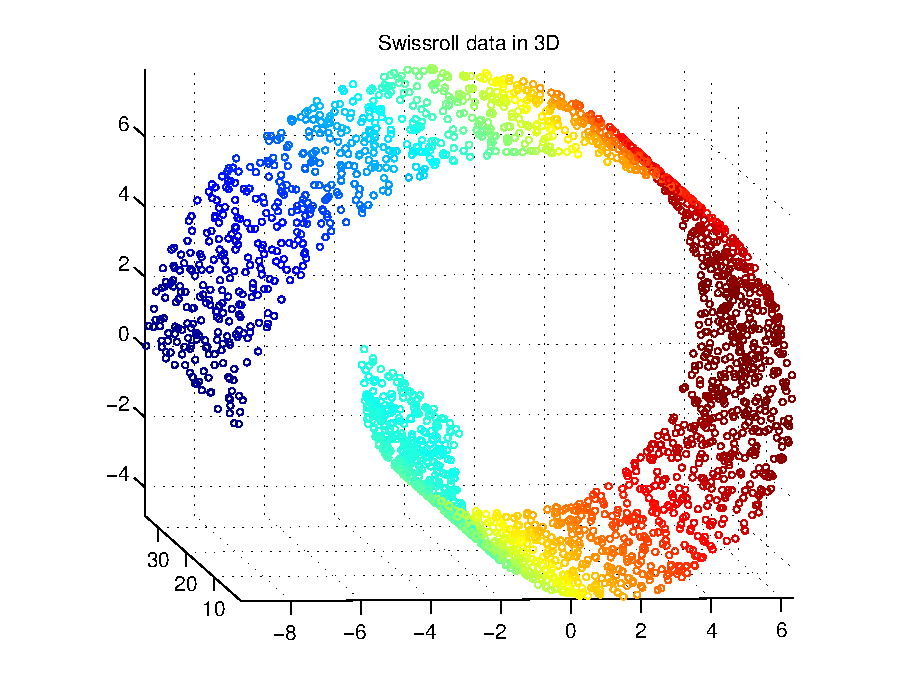
\includegraphics[width=.7\textwidth]{figures/swissroll_data.eps}
\caption{The sampled swissroll.}
\label{fig:swissroll}
\end{figure}

\subsection*{2.1 Swissroll}

Our original swissroll data (figure \ref{fig:swissroll}) consists of 2500 points randomly sampled from a 2D uniform distribution and then mapped to a swissroll by using the swissroll map:

\begin{equation}
 (X, Y) \rightarrow (X \cdot cos(X), Y, X\cdot sin(X))
\label{eq:swiss_map}
\end{equation}

This data is generated in \texttt{gen\_swissroll.m}. Our swissroll experiments can be reproduced fully by running the top-level script \texttt{swissroll.m}. Figure \ref{fig:swiss_embeddings} shows embeddings and eigenvalue magnitudes for various values of the parameter $k$. The eigenvalue magnitudes ``give away" the dominant dimensionality of the produced embedding. As can be witnessed by our results, the value of $k$ has
a tremendous effect on the embedding, both from a visual and a mathematical perspective. For $k=4$, we tend to favor a one-dimensional embedding. Also note that for small values of $k$ (in this case, $k < 7$) the $k$-nearest neighbor graph introduces multiple connected components. We take care of this by using MATLAB's connected component functionalities. For more details, we refer the reader to the comments of \texttt{swissroll.m}.

\begin{figure}
\centering
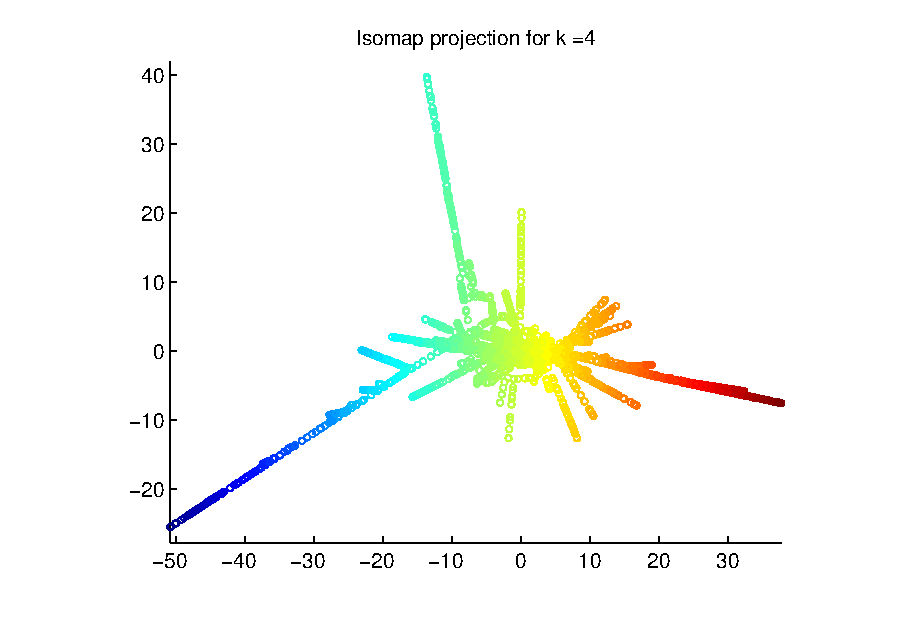
\includegraphics[width = .4\textwidth]{figures/swissroll_embedding_k=4}
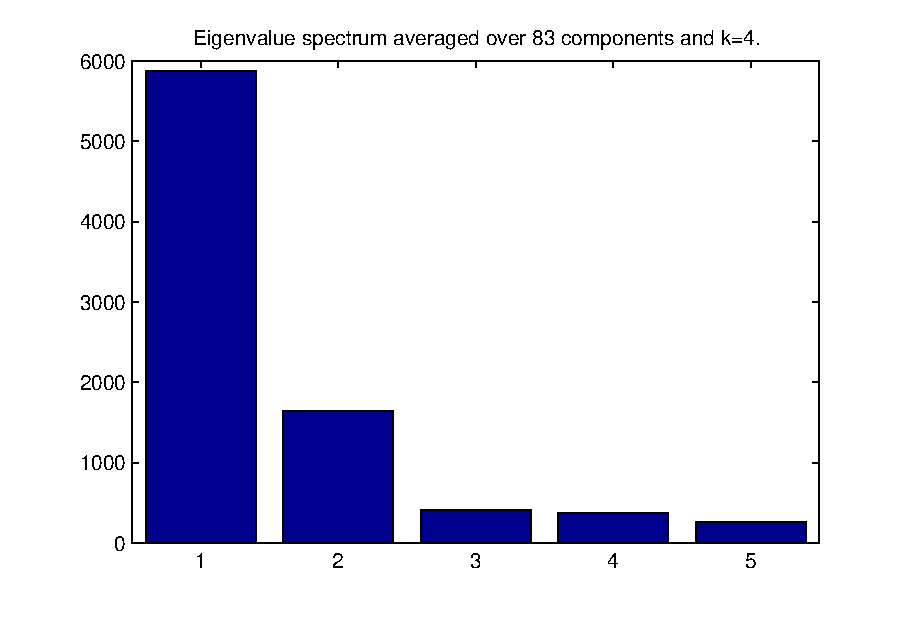
\includegraphics[width = .4\textwidth]{figures/swissroll_barplot_k=4}\\
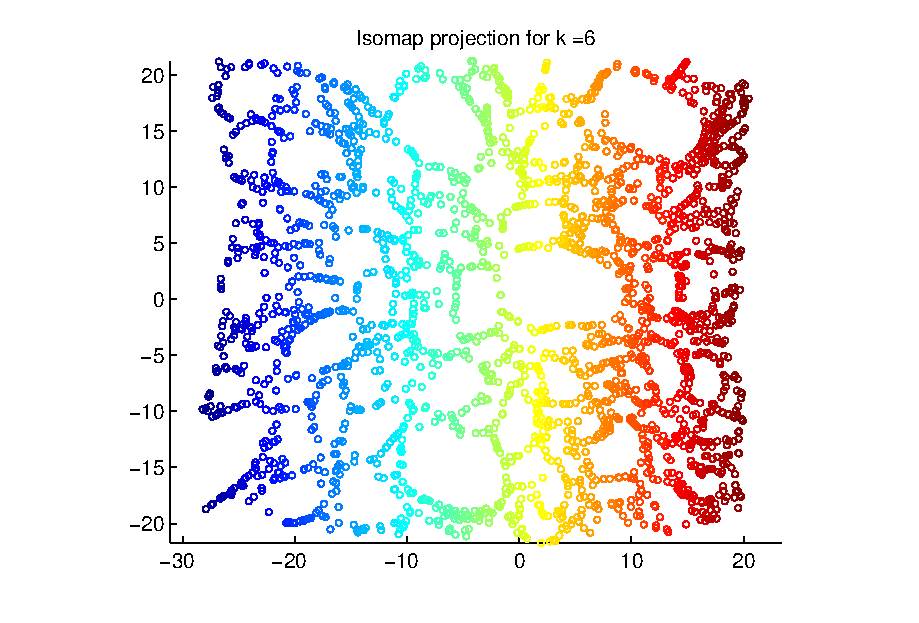
\includegraphics[width = .4\textwidth]{figures/swissroll_embedding_k=6}
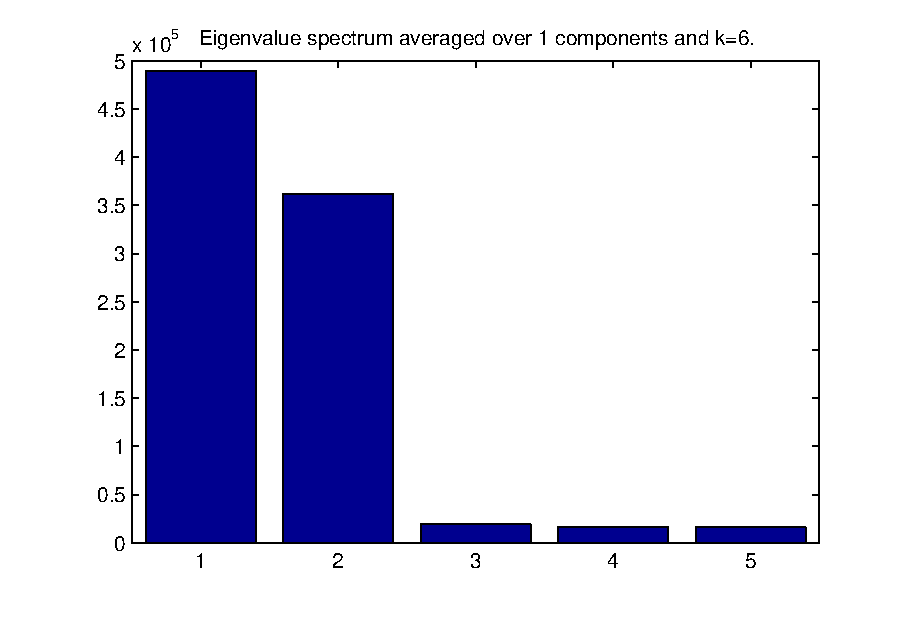
\includegraphics[width = .4\textwidth]{figures/swissroll_barplot_k=6} \\
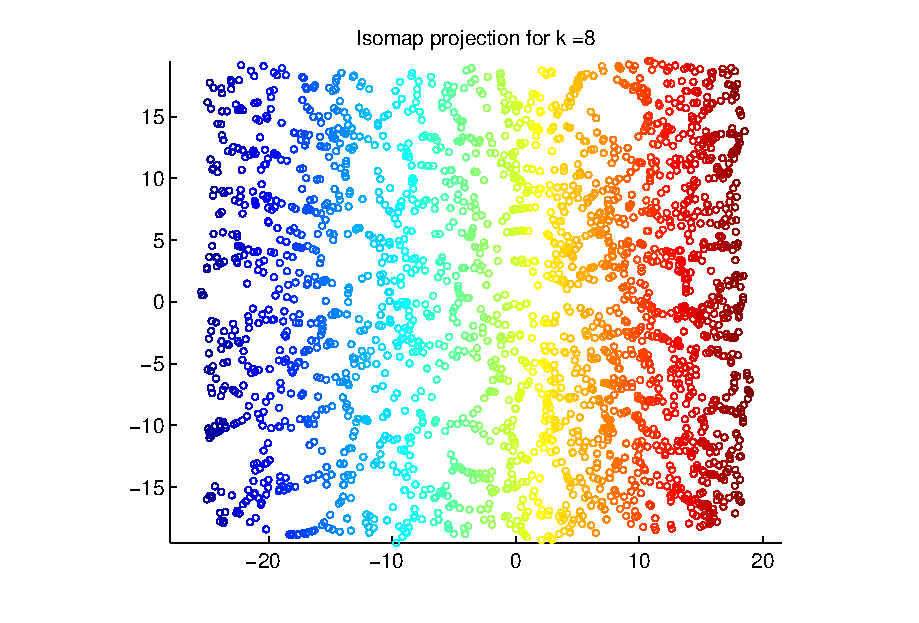
\includegraphics[width = .4\textwidth]{figures/swissroll_embedding_k=8}
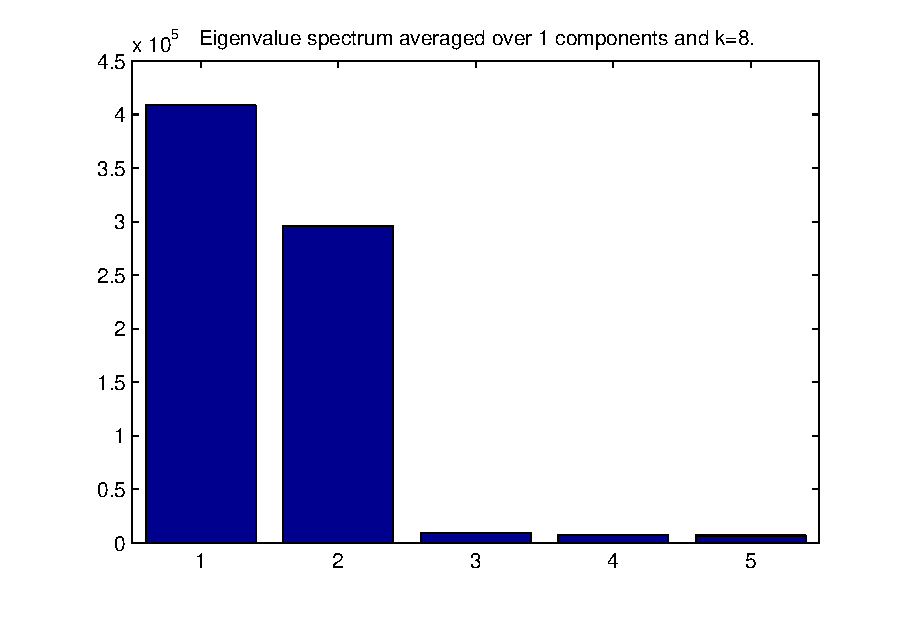
\includegraphics[width = .4\textwidth]{figures/swissroll_barplot_k=8}\\ 
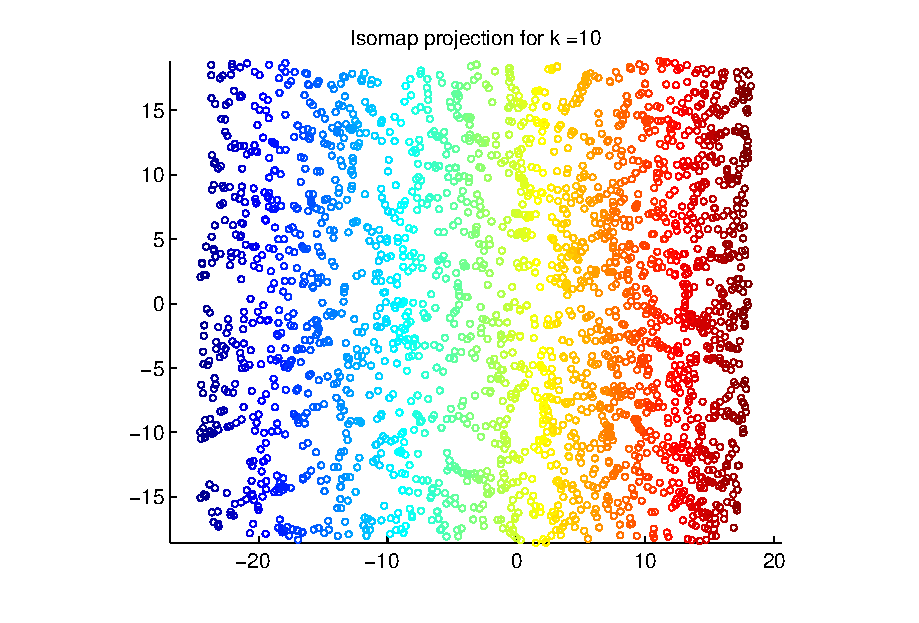
\includegraphics[width = .4\textwidth]{figures/swissroll_embedding_k=10}
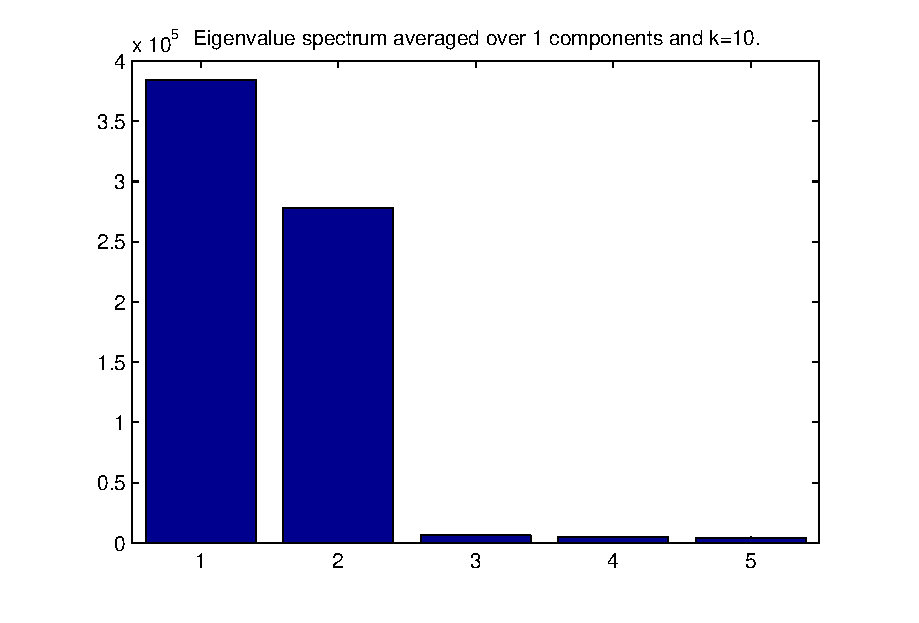
\includegraphics[width = .4\textwidth]{figures/swissroll_barplot_k=10}\\ 
\caption{Swissroll embeddings and eigenvalue spectra for $k=4, 6, 8,  10$.}
\label{fig:swiss_embeddings}
\end{figure}

For all $k > 4$, the eigenvalue spectrum still shows only 2 appreciable eigenvalues. This is understandable, since essentially our data
is nothing beyond a curved 2D plane in 3D.

\subsection*{2.2 Sinusoid}

The MATLAB function file \texttt{gen\_sinusoid.m} was used to generate a 2D sinusoid of 2000 points embedded in 3D (Figure \ref{fig:sinusoid}).  Figure 
\ref{fig:sinus_embeddings} shows the embeddings attained for this sinusoid for various values of $k$. We again see that $k$ has a direct consequence
on the form of the embedding. For $k=4$, we obtain an almost 1D embedding. For larger values of $k$, Isomap converges to the intrinsic dimensionality 
of the dataset. The results are reproducible by running the script \texttt{sinusoid.m}.

\begin{figure}
\centering
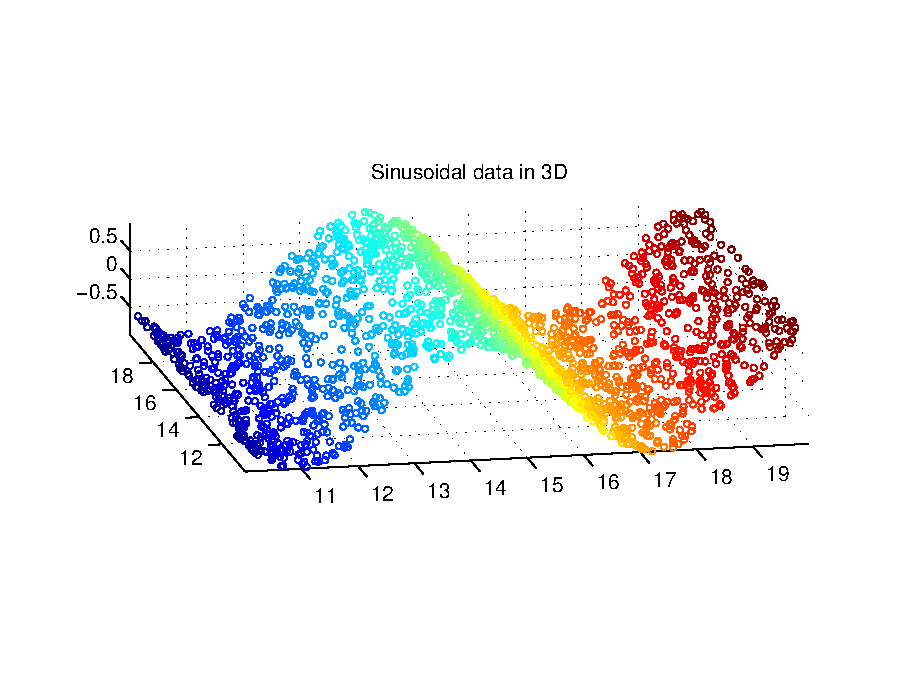
\includegraphics[width=.7\textwidth]{figures/sinusoid_data.eps}
\caption{The sampled sinusoid.}
\label{fig:sinusoid}
\end{figure}

\begin{figure}
\centering
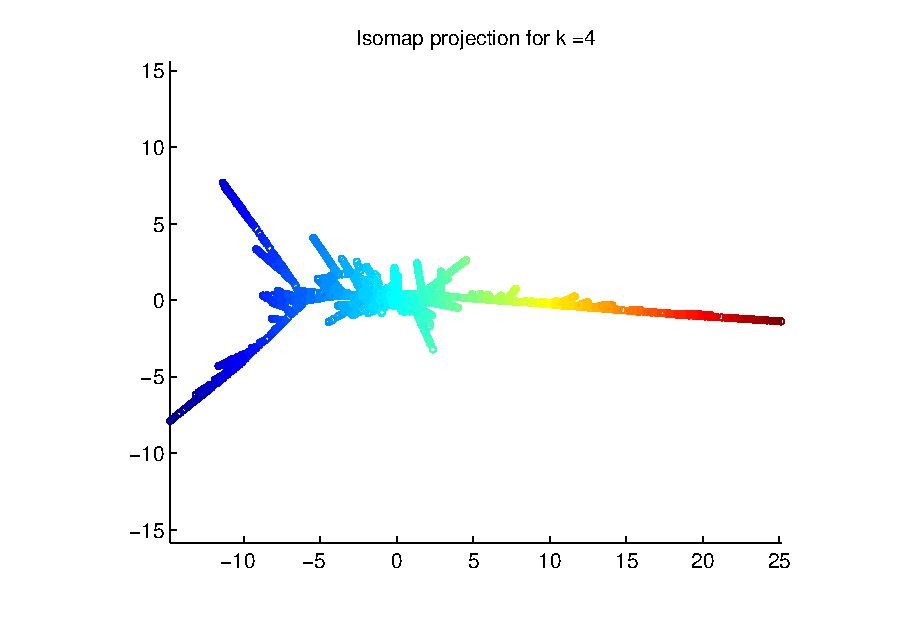
\includegraphics[width = .4\textwidth]{figures/sinusoid_embedding_k=4}
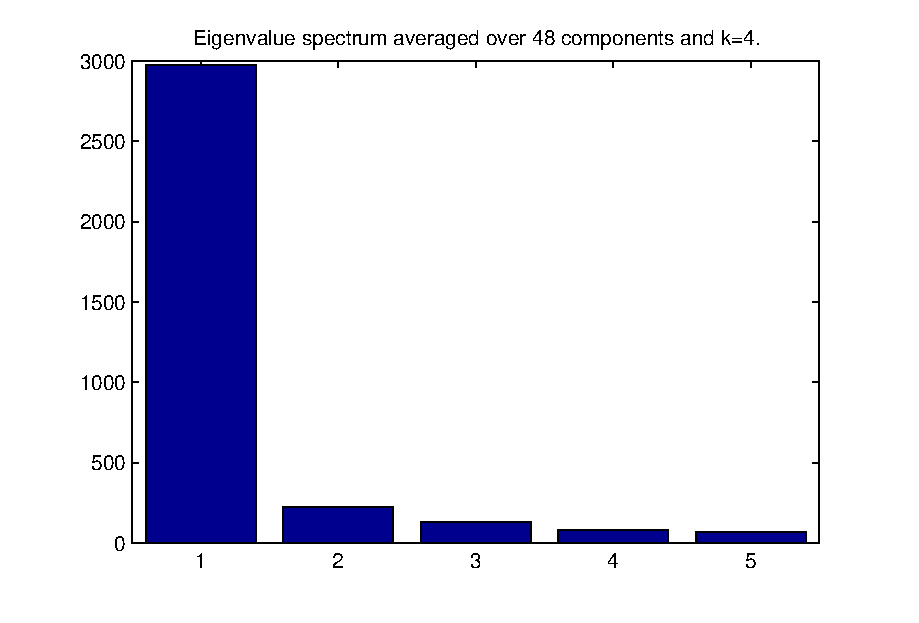
\includegraphics[width = .4\textwidth]{figures/sinusoid_barplot_k=4}\\
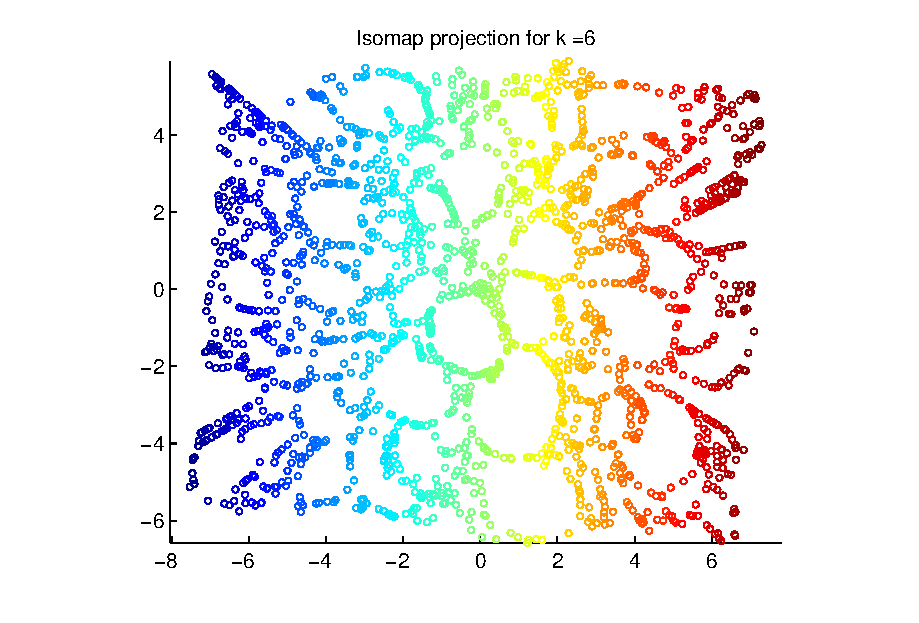
\includegraphics[width = .4\textwidth]{figures/sinusoid_embedding_k=6}
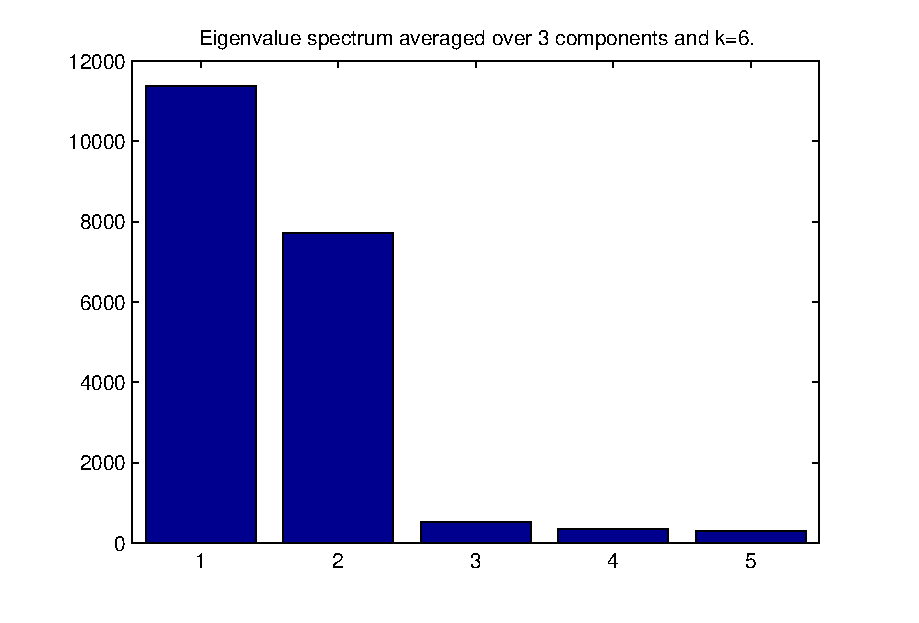
\includegraphics[width = .4\textwidth]{figures/sinusoid_barplot_k=6} \\
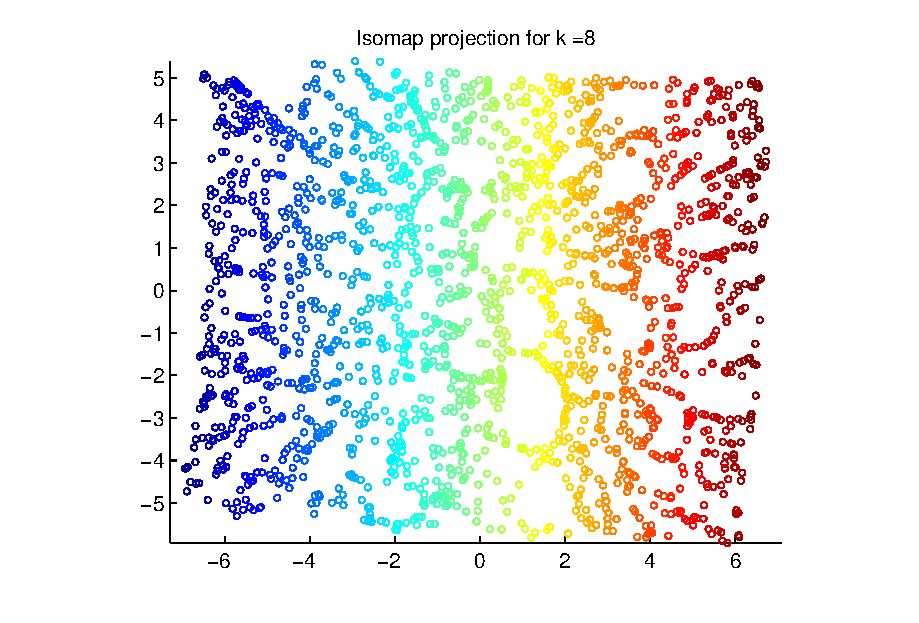
\includegraphics[width = .4\textwidth]{figures/sinusoid_embedding_k=8}
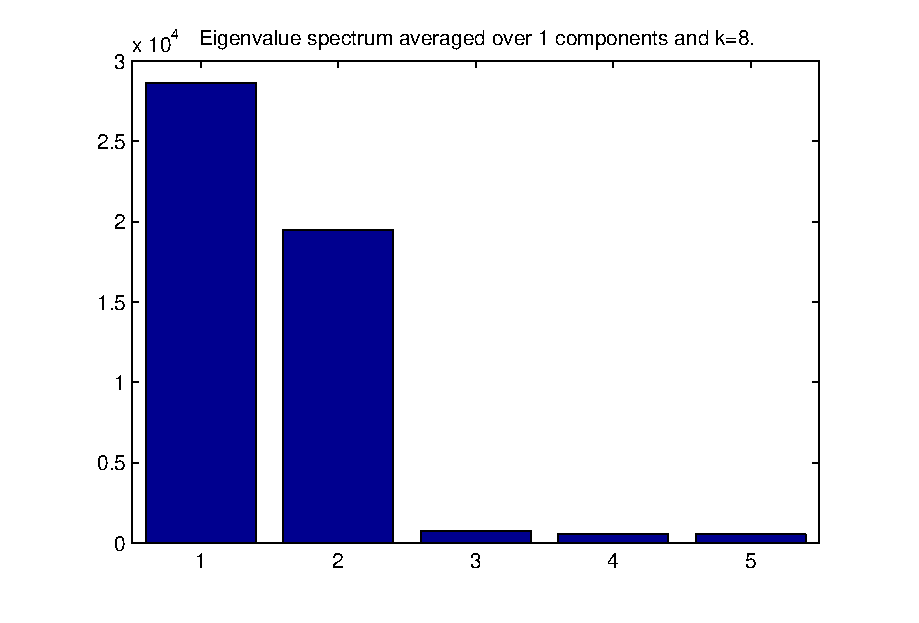
\includegraphics[width = .4\textwidth]{figures/sinusoid_barplot_k=8}\\ 
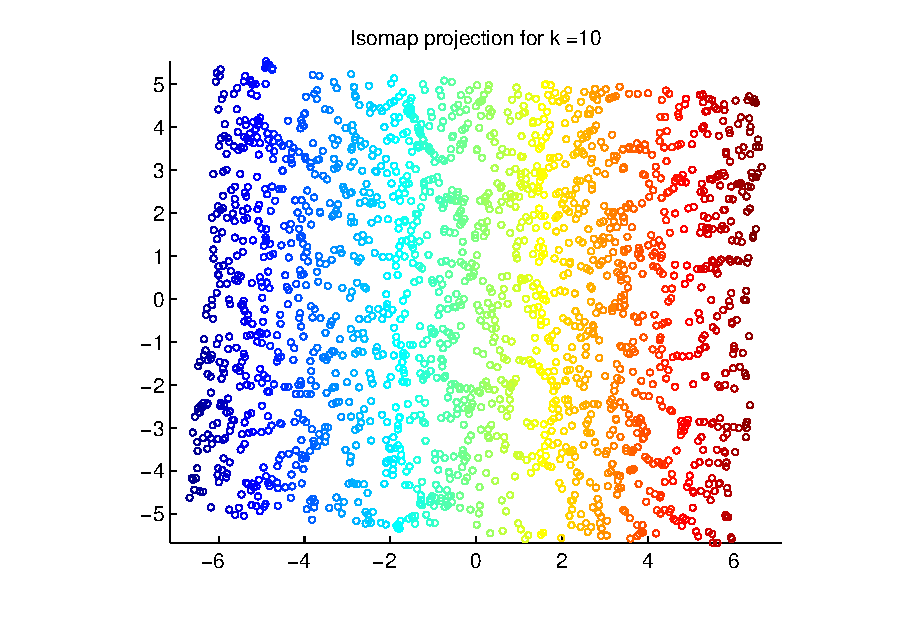
\includegraphics[width = .4\textwidth]{figures/sinusoid_embedding_k=10}
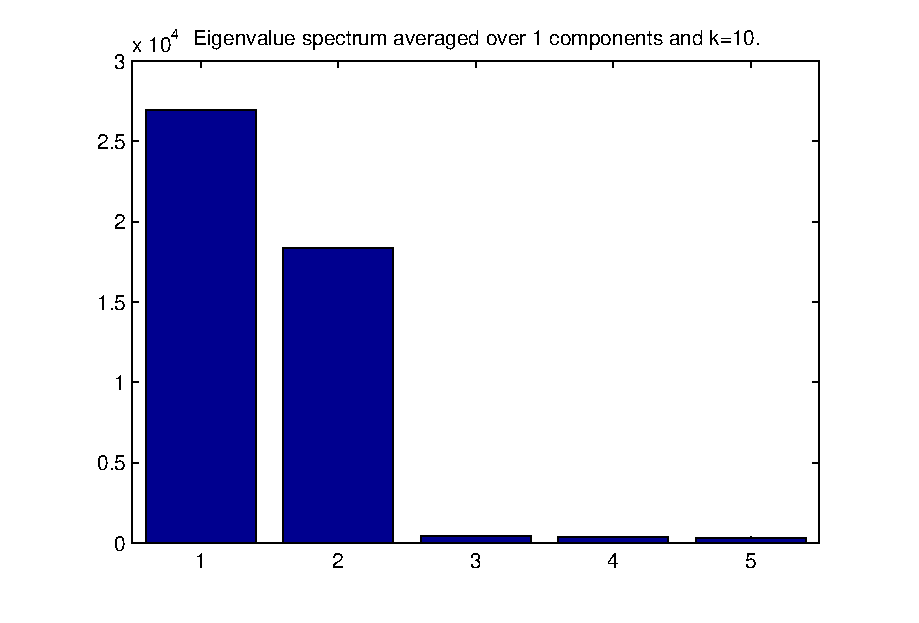
\includegraphics[width = .4\textwidth]{figures/sinusoid_barplot_k=10}\\ 
\caption{Sinusoid embeddings and eigenvalue spectra for $k=4, 6, 8,  10$.}
\label{fig:sinus_embeddings}
\end{figure}

\section*{3. Face data}

Finally, we apply our implementation of Isomap to the face data used in \cite{Tenenbaum2000}, downloadable from \url{
http://isomap.stanford.edu/}. This data consists of 698 grayscale images of the same face, with rotations along the X and Y axis and variation in 
lighting. These degrees of freedom are the dominant ones in this dataset, which is used as one of the running examples of \cite{Tenenbaum2000}.
The authors have been able to recover these degrees of freedom through the eigenvalue spectrum returned by Isomap, and as can be made evident by 
figure \ref{fig:faceDataSpectra}, so can our own implementation of the algorithm. It should be pointed out that the 4th and 5th eigenvalues are not
significantly smaller than the 3rd: this mirrors the experimental results of \cite{Tenenbaum2000} and reflects the fact that the degrees of freedom are 
distorted by phenomena such as self-shadowing and non-symmetries in the face. Running the script \texttt{expFaceData.m} reproduces our results.

\begin{figure}
\centering
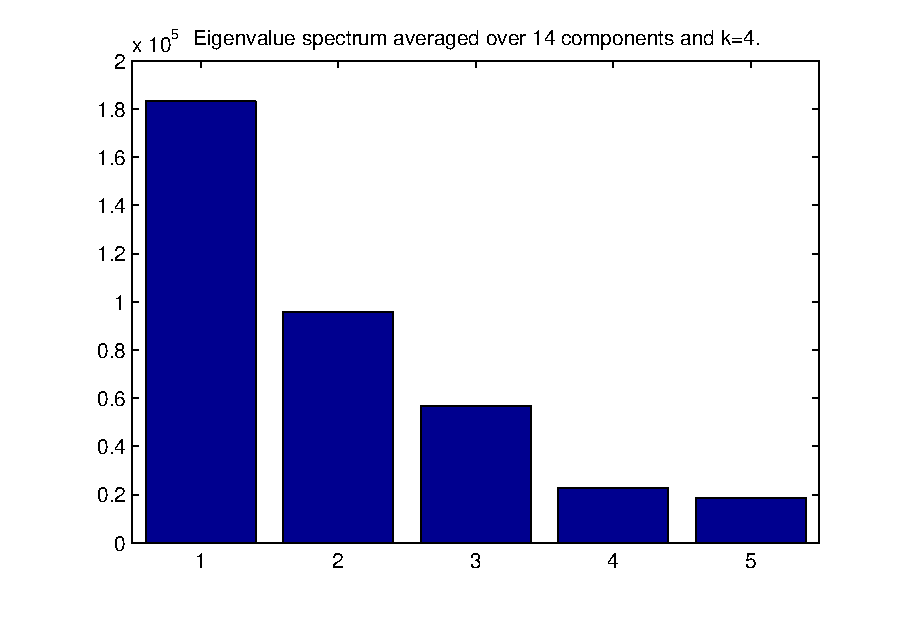
\includegraphics[width=.4\textwidth]{figures/faceEigSpectrum_k=4}
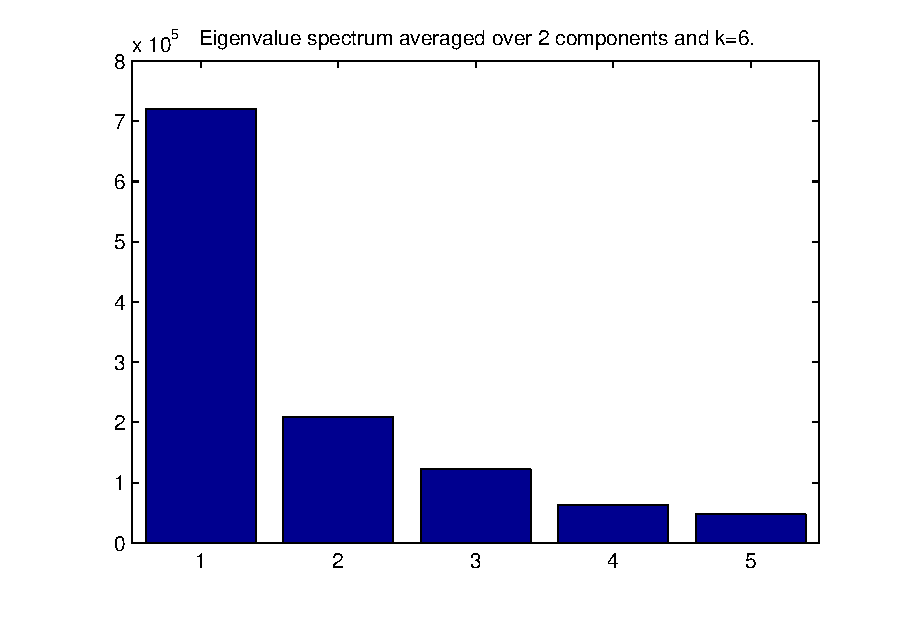
\includegraphics[width=.4\textwidth]{figures/faceEigSpectrum_k=6}\\
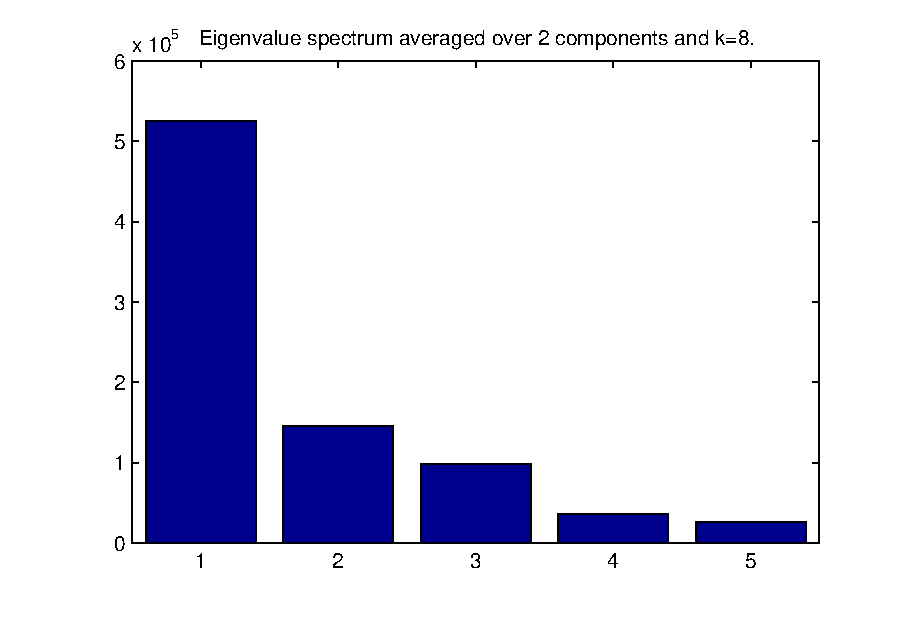
\includegraphics[width=.4\textwidth]{figures/faceEigSpectrum_k=8}
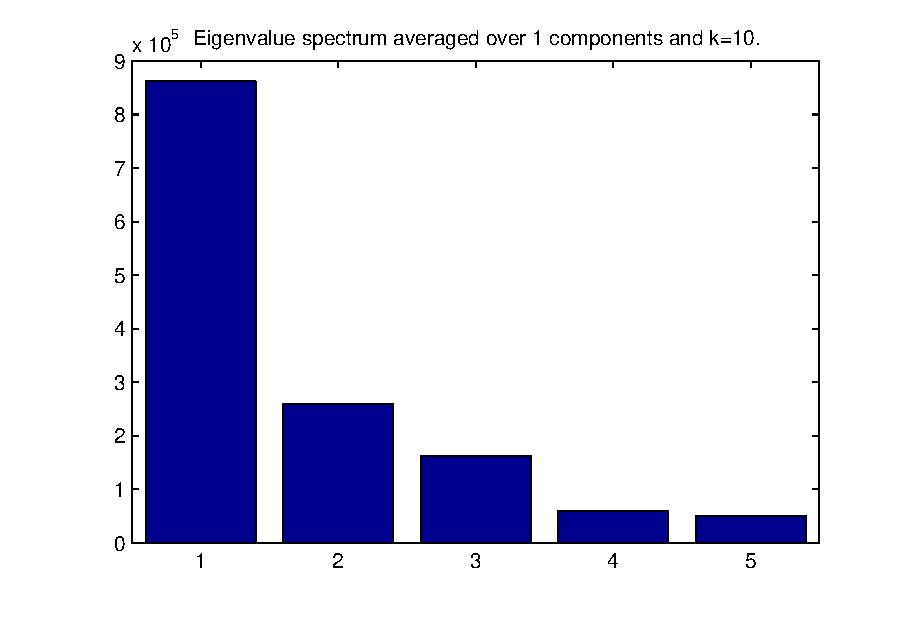
\includegraphics[width=.4\textwidth]{figures/faceEigSpectrum_k=10}
\caption{Face data eigenvalue spectra for $k=4, 6, 8, 10$.}
\label{fig:faceDataSpectra}
\end{figure}

\section*{4. Conclusions}

In this project, we implemented Isomap, the original and most widely used algorithm for Manifold Learning. We showed the steps of Isomap
and hinted towards code snippets that implement those steps. We experimented on synthetic and real data and found that the results matched our
intuitions (for the synthetic data) as well as prior, published results (for the real data).

Isomap has been terrifically studied in the manifold literature and most of its theoretical strengths and weaknesses have been discussed. With this work,
we aimed to address some practical challenges that an implementation of this algorithm needs to address. Specifically:

\begin{enumerate}
\item We deal with the issue of multiple connected components more thoroughly than the original Isomap implementation, which was only capable of
projecting one connected component, whenever multiple exist. We find that this issue is prevalent in sparsely sampled data or when the value of $k$ is
small. For example, for $k=4$, the 4-nearest neighbor graph produced for our densely sampled ($N=2500$) swissroll introduced 36 connected components.

\item We perform a visual and mathematical examination of the effect that the parameter $k$ has on the form of the embeddings produced. We determine that, if $k$ is not ``sufficiently" large, the data tends to be projected in a linear subspace of lower dimensionality than the intrinsic dimensionality of the data. In cases where the user has some prior information about this intrinsic dimensionality (e.g face data), then tuning $k$ such
that this dimensionality is well-reflected is possible. However, in the general case, where there is no prior information about the manifold whatsoever,
it does not seem obvious how $k$ should be selected. To the best of our knowledge, there do not exist theoretical guarantees that link the value of $k$ to the intrinsic dimensionality of the dataset.

\item We experimentally verify that the biggest bottleneck behind Isomap is the shortest-path algorithm runtime. An original implementation used Dijkstra's algorithm and iterated over half the nodes in the structure, for a total complexity of $O({{N}\choose{2}}\times log(N)\times E)$, where $N$ is the number of nodes and $E$ is the number of edges in the graph. As the value of $k$ increases, $E$ explodes, leading to complications with this algorithm selection. We substitute our use of Dijkstra's algorithm through $\texttt{graphshortestpath}$ to Johnson's algorithm, through $\texttt{graphallshortestpaths}$, which provides for a complexity that only depends linearly on $E$: $O(N\times log(N) + N \times E)$. Furthermore,
our implementation is easily parallelizable by using MATLAB's \texttt{parfor} loops such that multiple values of $k$ are tested simultaneously. One would only need to take one of the three top-level scripts, add
\texttt{matlabpool(n)} with \texttt{n} the required number of MATLAB workers (processing threads) before the for loops, change the for loops into parfor loops and add \texttt{matlabpool close} after the loops. Prior to employing Johnson's algorithm, this is how we structured these scripts; after using Johnson, the computational benefit was so significant that there did not exist good reason to burden the host machine's threads with parallel computation.
\end{enumerate}


\bibliography{../828_refs}
\bibliographystyle{plain}
\end{document}
